\subsection{BPMN diagrama} \label{section:bpmn}
Norint standartizuoti verslo modelių atvaizdavimą 2004 metais organizacija BPMI išleido \BPMN{} 1.0 specifikaciją. Ji leido tiek vaizduoti esamus, tiek apsikeisti kuriamų procesų reikalavimais. \BPMN{} greitai išpopuliarėjo tarp vadybininkų, verslo analitikų ir programuotojų, nes pasiūlė pažįstamą verslo procesų atvaizdavimą ir turėjo matematinį pagrindą. Vėliau BPMI susijungė su \OMG{} ir 2013 metais buvo išleista \BPMN{} 2.0 versija, kurioje \BPMN{} įgavo geresnį skaitomumą, lankstumą ir išplečiamumą.

\subsubsection{BPMN apimtis}
\BPMN{} specifikacija standartizuoja verslo procesų modelį, jų atvaizdavimo būdą ir duomenų apsikeitimo formatą perduoti tiek modelį, tiek jo atvaizdavimą. Sutelkti dėmesiui į skirtingas proceso dalis pateikiami procesų ir choreografijos submodeliai. Bendradarbiavimo submodelis, į save įtraukiantis kitus, gali būti naudojamas pateikti iš karto viskam. Specifikacijos apimtis yra verslo procesai taigi dalykai kaip strategija, duomenų struktūros, resursai, taisyklės ir įstatymai neįeina į ją.

\subsubsection{BPMN komponentai} \label{section:bpmn_components}
\BPMN{} specifikacija leidžia atvaizduoti gana nemažai verslo proceso atributų \cite{bpmnFormal}. Specifikacijoje jie yra suskirstyti į pagrindinius ir išvestinius. Toliau pateikiami pagrindiniai \BPMN{} komponentai.

\begin{figure}[H]
	\centering
	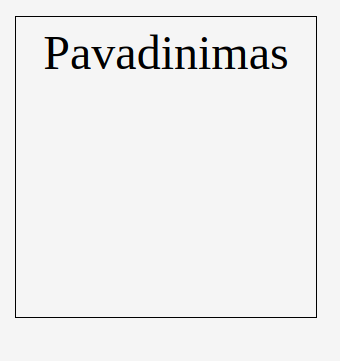
\includegraphics[width=5cm]{img/bpm-components/pool}
	\caption{Juostos žymėjimo pavyzdys}
	\label{img:bpm_components_pool}
\end{figure}

Juosta (pool) žymi diagramos dalyvį. Šio komponento paskirtis yra parodyti už kokias veiklas ir koks vykdytojas yra atsakingas. Juosta gali būti skaidoma smulkiau norint konkrečiau nurodyti vykdytojų grupes ir jų pareigas, tuomet ji gali būti vadinama linija (lane). Juosta žymima apibraukiant tam tikrą sritį (\ref{img:bpm_components_pool} pav.). Viduje yra vieta komponentams už kurių atlikimą atsakingas dalyvis.

\begin{figure}[H]
	\centering
	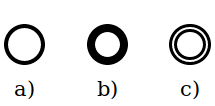
\includegraphics[width=5cm]{img/bpm-components/event_types}
	\caption{Įvykio žymėjimo pavyzdys}
	\label{img:bpm_event_types}
\end{figure}

Įvykis (event) žymi, kad įvyko kažkas, kas įtakojo proceso būseną. Šis komponentas dažniausiai turi priežastį (trigger) dėl ko jis įvyko ir pasekmes (result). Specifikacijoje įvykiai skirstomi į tris tipus: pradžios (\ref{img:bpm_event_types} pav. a), pabaigos (\ref{img:bpm_event_types} pav. b) ir tarpinius (\ref{img:bpm_event_types} pav. c). Žymėjimas yra tuščias apskritimas (\ref{img:bpm_event_types} pav.), viduje paliekant vietos tipo konkretizavimui.

\begin{figure}[H]
	\centering
	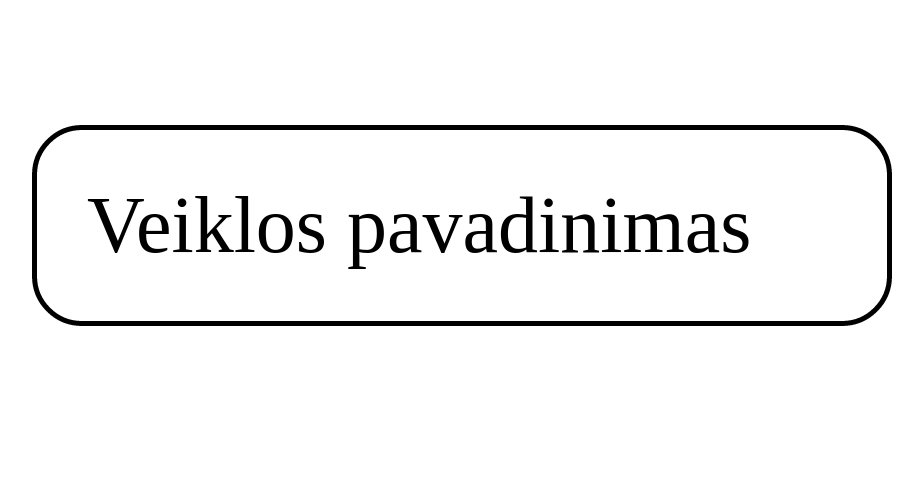
\includegraphics[width=5cm]{img/bpm-components/activity}
	\caption{Veiklos žymėjimo pavyzdys}
	\label{img:bpm_components_activity}
\end{figure}

Veikla (Activity) yra darbas atliekamas organizacijos procesuose. Ji gali būti atominė ir turėti tik pavadinimą arba  skaidoma labiau, tokiu būdu tapdama subprocesu. Visais atvejais žymėjimas yra stačiakampis su užapvalintais kampais (\ref{img:bpm_components_activity} pav.).

\begin{figure}[H]
	\centering
	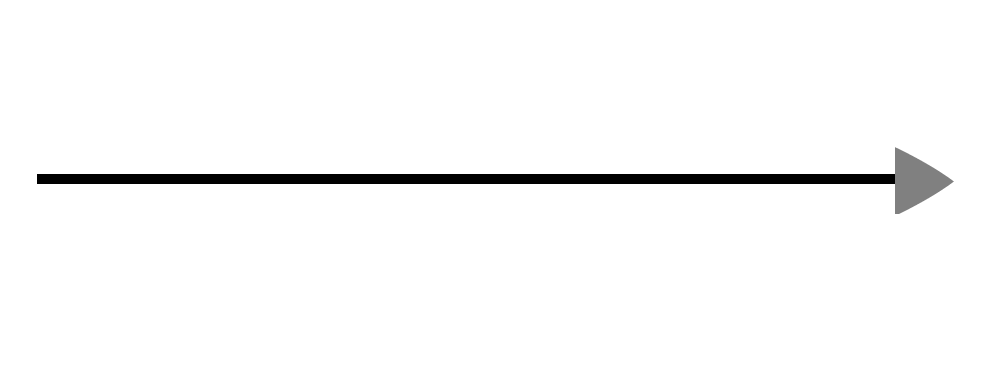
\includegraphics[width=5cm]{img/bpm-components/transition}
	\caption{Sekos srauto žymėjimo pavyzdys}
	\label{img:bpm_components_sequence_flow}
\end{figure}

Sekos srautas (Sequence Flow) žymi veiklų seką. Jeigu nenurodyta lygiagretumo veiklos modelyje vykdomos iš eilės. Šis komponentas parodo kokia tvarka tai vyks. Jį galima apibūdinti kaip grafo su kryptimis briauna, kryptis parodo kuri veikla turi būti įvykdyta vėliau. Sekos srautas žymimas solidžia linija ir užpildyto trikampio formos rodykle parodančia kryptį (\ref{img:bpm_components_sequence_flow} pav.).

\begin{figure}[H]
	\centering
	
\includegraphics[width=5cm]{img/bpm-components/gateway}
	\caption{Sprendimo žymėjimo pavyzdys}
	\label{img:bpm_components_gateway}
\end{figure}

Sprendimas (gateway) gali būti įterptas sekos srautuose tarp veiklų. Jis žymi srautų išsišakojimą arba susijungimą. Šis komponentas parodo, kad priklausomai nuo konkretaus proceso būsenos bus vykdomos veiklos į kurias eina sekos srautai atitinkantys sprendimo sąlygas. Žymėjimas yra kvadratas pasuktas 45 laipsniu kampu (\ref{img:bpm_components_gateway} pav.). Viduje yra vieta sprendimo konkretizavimui.

\begin{figure}[H]
	\centering
	
\includegraphics[width=5cm]{img/bpm-components/data_object}
	\caption{Duomenų objekto žymėjimo pavyzdys}
	\label{img:bpm_components_data_object}
\end{figure}

Duomenų objektas (data Object) pateikia informaciją apie tai kokių duomenų reikalauja veiklos vykdytojas norėdamas ją atlikti ir kokie duomenys pagaminami po jos vykdymo. Komponentas gali žymėti tiek neskaidomus tiek sudėtinius duomenis. Jis vaizduojamas (\ref{img:bpm_components_data_object} pav.) kaip stačiakampis su nukirptu dešiniuoju viršutiniu kampu ir trikampiu prie jo (arba kaip stačiakampis lapas su užlenktu dešiniuoju viršutiniu kampu).

\begin{figure}[H]
	\centering
	
\includegraphics[width=5cm]{img/bpm-components/message}
	\caption{Pranešimo žymėjimo pavyzdys}
	\label{img:bpm_components_message}
\end{figure}

Pranešimas (message) žymi bendravimą tarp dalyviu. Šis komponentas skirtas apibrėžti perduodamai informacijai tarp jų. Vaizduojamas (\ref{img:bpm_components_message} pav.) stačiakampiu su trikampiu viduje (vokas).

\begin{figure}[H]
	\centering
	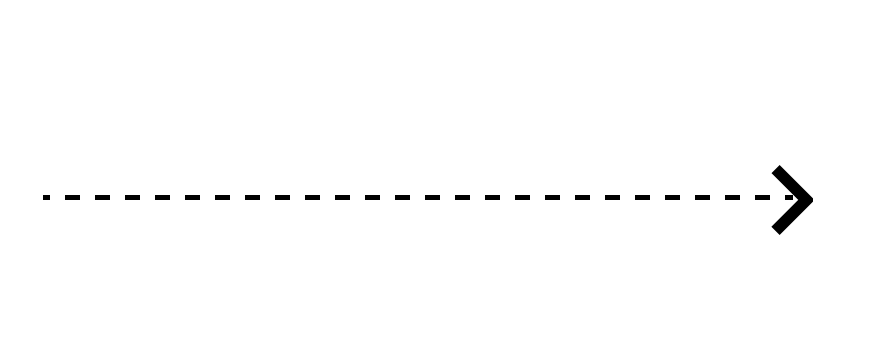
\includegraphics[width=5cm]{img/bpm-components/message_flow}
	\caption{Pranešimų srauto žymėjimo pavyzdys}
	\label{img:bpm_components_message_flow}
\end{figure}

Pranešimų srautas (Message flow) žymi duomenų perdavimą. Tai yra kryptinė grafo briauna, kuri jungia duomenų objektus ir žinutes su juos sukuriančiomis arba naudojančiomis veiklomis. Duomenų srautas į objektą ar žinutę rodo, kad tai yra veiklos išeiga, priešingu atveju tai yra veiklos įeiga, duomenys reikalingi jai įvykdyti. Vaizduojama (\ref{img:bpm_components_message} pav.) punktyrine linija su rodykle rodančia kryptį.

\begin{figure}[H]
	\centering
	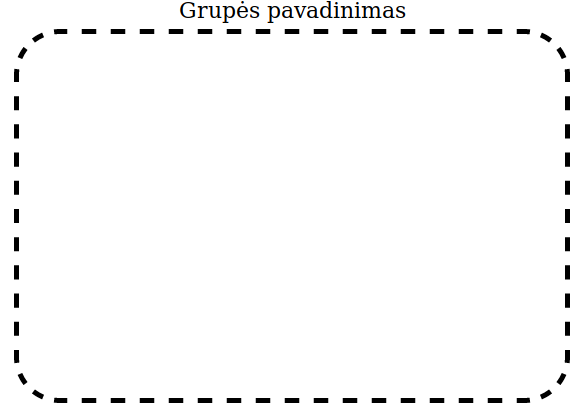
\includegraphics[width=5cm]{img/bpm-components/group}
	\caption{Grupės žymėjimo pavyzdys}
	\label{img:bpm_components_group}
\end{figure}

Grupė (group) skirta nurodyti modelio komponentų kategorijas. Ji neturi įtakos sekų ar duomenų srautams, o tik pasako kas priklauso tai pačiai kategorijai. Vaizdavimas diagramoje yra komponentų apibraukimas ir grupės pavadinimo nurodymas (\ref{img:bpm_components_group} pav.).

\begin{figure}[H]
	\centering
	
\includegraphics[width=5cm]{img/bpm-components/text_annotation}
	\caption{Komentaro žymėjimo pavyzdys}
	\label{img:bpm_components_text_annotation}
\end{figure}

Komentaras (text annotation) yra mechanizmas skirtas pateikti papildomai informacijai diagramos skaitytojams. Šis komponentas neįtakoja sekos ar duomenų srautų, o tik paaiškina kas ir kodėl vyksta. Žymimas skliaustu iš kairės komentaro teksto pusės (\ref{img:bpm_components_text_annotation} pav.).

\begin{figure}[H]
	\centering
	
\includegraphics[width=5cm]{img/bpm-components/association}
	\caption{Asociacijos žymėjimo pavyzdys}
	\label{img:bpm_components_text_association}
\end{figure}

Asociacija (association) skirta komentarams susieti su modelio komponentais. Ji nurodo kuri diagramos dalis yra komentuojama. Asociacija vaizduojama punktyrine linija (\ref{img:bpm_components_text_association} pav.).

\subsubsection{BPMN komponentų tarpusavio ryšiai}
Norint modeliuoti verslo procesus vien komponentų nepakanka, taip pat reikia žinoti ir kaip jie sąveikauja tarpusavyje. Tarpusavio ryšius gana neblogai apibūdina metamodelis. Šiame darbe jis bus dažnai naudojamas tam tikslui. Skyriuje \ref{section:bpmn_components} aprašytų komponentų sąveiką galima pavaizduoti (\ref{img:bpmn_metamodel} pav.) metamodeliu.

\begin{figure}[H]
	\centering
	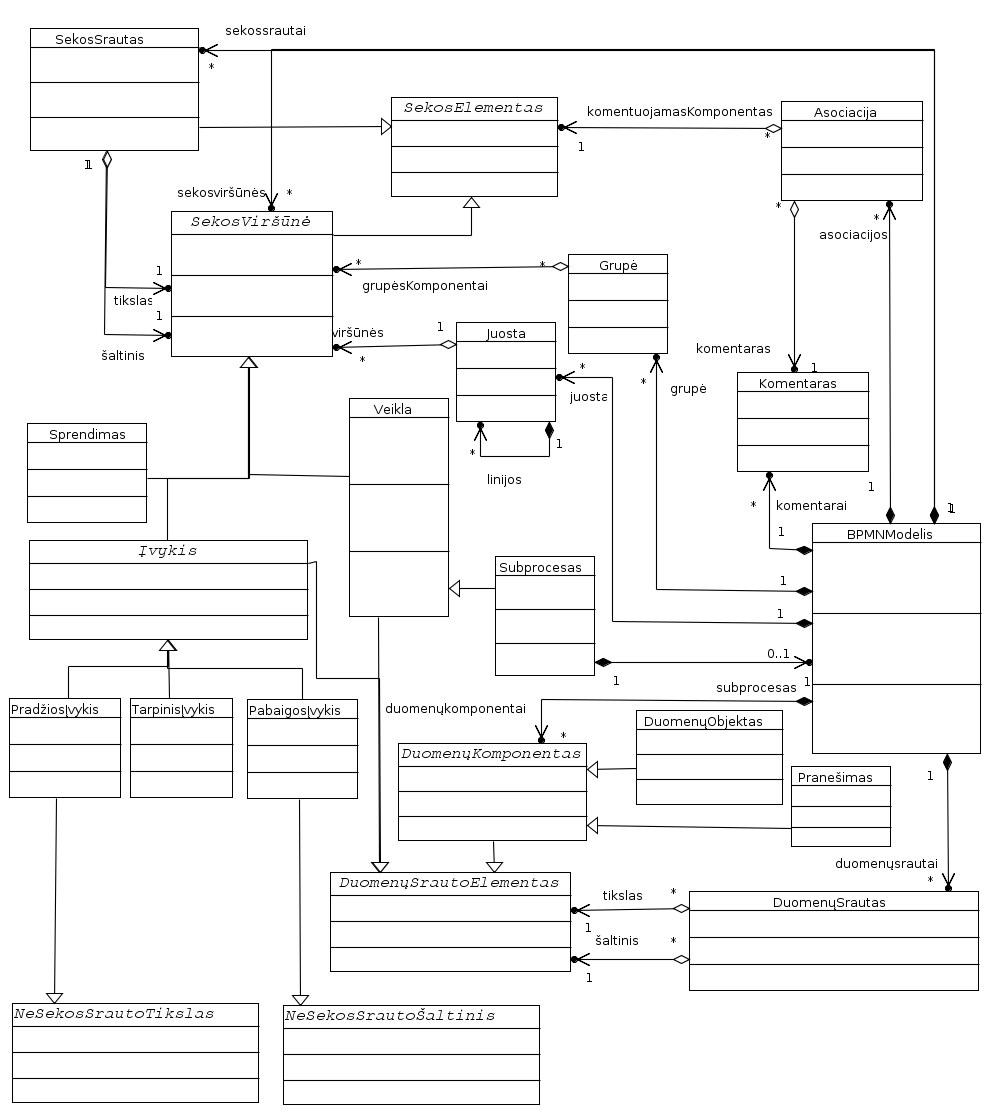
\includegraphics[width=\textwidth]{sections/modeling_methods_and_languages/img/bpmn_metamodel}
	\caption{\BPMN{} pagrindinių komponentų metamodelis}
	\label{img:bpmn_metamodel}
\end{figure}

Šiame metamodelyje tipas BPMNModelis yra šakninis komponentas. Jis savyje laiko
sekos viršūnes, sekos srautus, juostas, grupes, duomenų komponentus, duomenų
srautus, komentarus ir asociacijas. Komponentus metamodelyje galima suskirstyti
į tris grupes: sekos komponentus, duomenų komponentus ir komentavimo komponentus.
Sekos komponentams priklauso SekosElemento tipų hierarchija, duomenų
komponentams priklauso DuomenųKomponento hierarchija ir DuomenųSrautas,
komentavimui priklauso Komentaras ir Asociacija. Taigi galima iš eilės
apibūdinti šias grupes iš kurių susideda \BPMN{} modelis.

Sekos viršūnė yra abstrakcija nurodanti, kad tai yra komponentai jungiami
sekos srautais, tokie kaip veikla, sprendimas ir įvykio subtipai. Įvykis yra
abstraktus tipas nes modelyje būna kurie nors iš jo subtipų. Sekos srautas turi
vieną šaltinį ir vieną tikslą. Autorius įveda 2 abstrakcijas: ne sekos srauto
šaltinis ir ne sekos srauto tikslas, kad parodyti \BPMN{} apribojimus, kurie
draudžia pabaigos įvykiui būti sekos srauto šaltiniu, o pradžios įvykiui –
tikslu.  Grupės ir Juostos nurodo kurios sekos viršunės joms priklauso.
Juosta dar gali turėti linijų. Metamodelyje taip pat parodoma, kad Veikla gali
būti subprocesas, tokiu būdu savyje laikydama kitą procesą. Duomenų srauto
elementas yra autoriaus įvesta abstrakcija parodanti, kad jo subtipai gali
būti jungiami duomenų srautais. Įvesta abstrakcija duomenų komponentas norint
apibendrinti praneŠimą ir duomenų objektą. Komentaras jungiamas Asociacija ir
gali komentuoti sekos komponentus.
